\documentclass[11pt,a4paper]{article}
\usepackage[utf8]{inputenc}
\usepackage{amsmath,amsfonts,amssymb}
\usepackage{graphicx}
\usepackage{geometry}
\geometry{margin=1in}
\usepackage{booktabs}
\usepackage{hyperref}
\usepackage{float}
\usepackage{xcolor}

\title{\textbf{EE3621: Digital Signal Processing} \\ \Large Lecture 24: Linear Prediction \& Vocoder / Speech Processing \\ \large (III B.Tech EEE)}
\author{Lecture Notes (40-Minute Plan)}
\date{}

\definecolor{darkbg}{HTML}{0d121f}
\definecolor{lighttext}{HTML}{e2e8f0}
\definecolor{primary}{HTML}{8b5cf6}
\definecolor{secondary}{HTML}{0dd5c5}

\pagecolor{darkbg}
\color{lighttext}

\hypersetup{
    colorlinks=true,
    linkcolor=secondary,
    urlcolor=secondary
}

\begin{document}

\maketitle

\section{Lecture Plan (40 Minutes Breakdown)}
\begin{itemize}
    \item \textbf{00:00 -- 06:00 (6 mins):} \textbf{Speech Production Model}: Source-filter model; glottal excitation vs white noise; vocal tract as all-pole filter.
    \item \textbf{06:00 -- 12:00 (6 mins):} \textbf{Linear Prediction (LP)}: Predict $x[n]$ from past $p$ samples; minimize prediction error.
    \item \textbf{12:00 -- 18:00 (6 mins):} \textbf{Normal (Yule-Walker) Equations}: Derivation; Toeplitz matrix structure.
    \item \textbf{18:00 -- 24:00 (6 mins):} \textbf{Levinson-Durbin Algorithm}: $O(p^2)$ recursive solution; PARCOR stability.
    \item \textbf{24:00 -- 30:00 (6 mins):} \textbf{LPC Vocoder}: Analysis/Synthesis, voiced/unvoiced, low bit rate.
    \item \textbf{30:00 -- 35:00 (5 mins):} \textbf{Cepstrum \& MFCCs}: Homomorphic analysis, log-spectrum, Mel scale.
    \item \textbf{35:00 -- 40:00 (5 mins):} \textbf{Pitch Detection Algorithms}: Autocorrelation, AMDF; Checkpoints.
\end{itemize}

\noindent\rule{\textwidth}{0.5pt}

\section{Speech Production Model}
The physical process of human speech generation can be approximated by the \textbf{Source-Filter Model}.

\subsection{Excitation Source}
\begin{itemize}
    \item \textbf{Voiced Speech:} Periodic vibration of vocal cords, modeled as a quasi-periodic impulse train with pitch period $T_0$.
    \item \textbf{Unvoiced Speech:} Modeled as random white noise (turbulence).
\end{itemize}

\subsection{Vocal Tract Filter}
Modeled as an \textbf{all-pole filter} $H(z)$:
\begin{equation}
H(z) = \frac{G}{1 + \sum_{k=1}^{p} a_k z^{-k}}
\end{equation}
The poles correspond to resonant frequencies (\textbf{formants}).

\section{Linear Prediction (LP) Formulation}
Predict sample $\hat{x}[n]$ from $p$ past samples:
\begin{equation}
\hat{x}[n] = -\sum_{k=1}^{p} a_k x[n-k]
\end{equation}
The prediction error is:
\begin{equation}
e[n] = x[n] - \hat{x}[n] = x[n] + \sum_{k=1}^{p} a_k x[n-k]
\end{equation}
Minimize mean squared error: $J = E\{e^2[n]\}$.

\section{Normal (Yule-Walker) Equations}
To minimize $J$, set partial derivatives to zero:
\begin{align}
\frac{\partial J}{\partial a_m} &= E\left\{ 2 \left( x[n] + \sum_{k=1}^{p} a_k x[n-k] \right) x[n-m] \right\} = 0 \\
\implies & E\{ x[n]x[n-m] \} + \sum_{k=1}^{p} a_k E\{ x[n-k]x[n-m] \} = 0
\end{align}
Using autocorrelation $R_{xx}[m] = E\{x[n]x[n-m]\}$:
\begin{equation}
\sum_{k=1}^{p} a_k R_{xx}[m-k] = -R_{xx}[m] \quad \text{for } m = 1, \dots, p
\end{equation}

Matrix form $\mathbf{R}\mathbf{a} = -\mathbf{r}$:
\begin{equation}
\begin{bmatrix}
R_{xx}[0] & R_{xx}[1] & \cdots & R_{xx}[p-1] \\
R_{xx}[1] & R_{xx}[0] & \cdots & R_{xx}[p-2] \\
\vdots & \vdots & \ddots & \vdots \\
R_{xx}[p-1] & R_{xx}[p-2] & \cdots & R_{xx}[0]
\end{bmatrix}
\begin{bmatrix}
a_1 \\ a_2 \\ \vdots \\ a_p
\end{bmatrix}
= -
\begin{bmatrix}
R_{xx}[1] \\ R_{xx}[2] \\ \vdots \\ R_{xx}[p]
\end{bmatrix}
\end{equation}

\section{Levinson-Durbin Algorithm}
Solves the Toeplitz system in $O(p^2)$ operations.
\begin{align}
E_0 &= R_{xx}[0] \\
k_1 &= -\frac{R_{xx}[1]}{E_0} \\
a_1^{(1)} &= k_1 \\
E_1 &= (1 - k_1^2) E_0
\end{align}
Update for $m = 1, \dots, p-1$:
\begin{align}
k_{m+1} &= -\frac{R_{xx}[m+1] + \sum_{i=1}^{m} a_i^{(m)} R_{xx}[m+1-i]}{E_m} \\
a_{m+1}^{(m+1)} &= k_{m+1} \\
a_i^{(m+1)} &= a_i^{(m)} + k_{m+1} a_{m+1-i}^{(m)} \\
E_{m+1} &= (1 - k_{m+1}^2) E_m
\end{align}
Stability is guaranteed if $|k_m| < 1$ for all $m$.

\section{LPC Vocoder}
\textbf{Analysis:} Extract $a_k$, Gain $G$, Pitch $T_0$, Voiced/Unvoiced flag. Transmit at ~2400 bps.
\textbf{Synthesis:} Reconstruct excitation and filter through $H(z)$.

\begin{figure}[H]
\centering
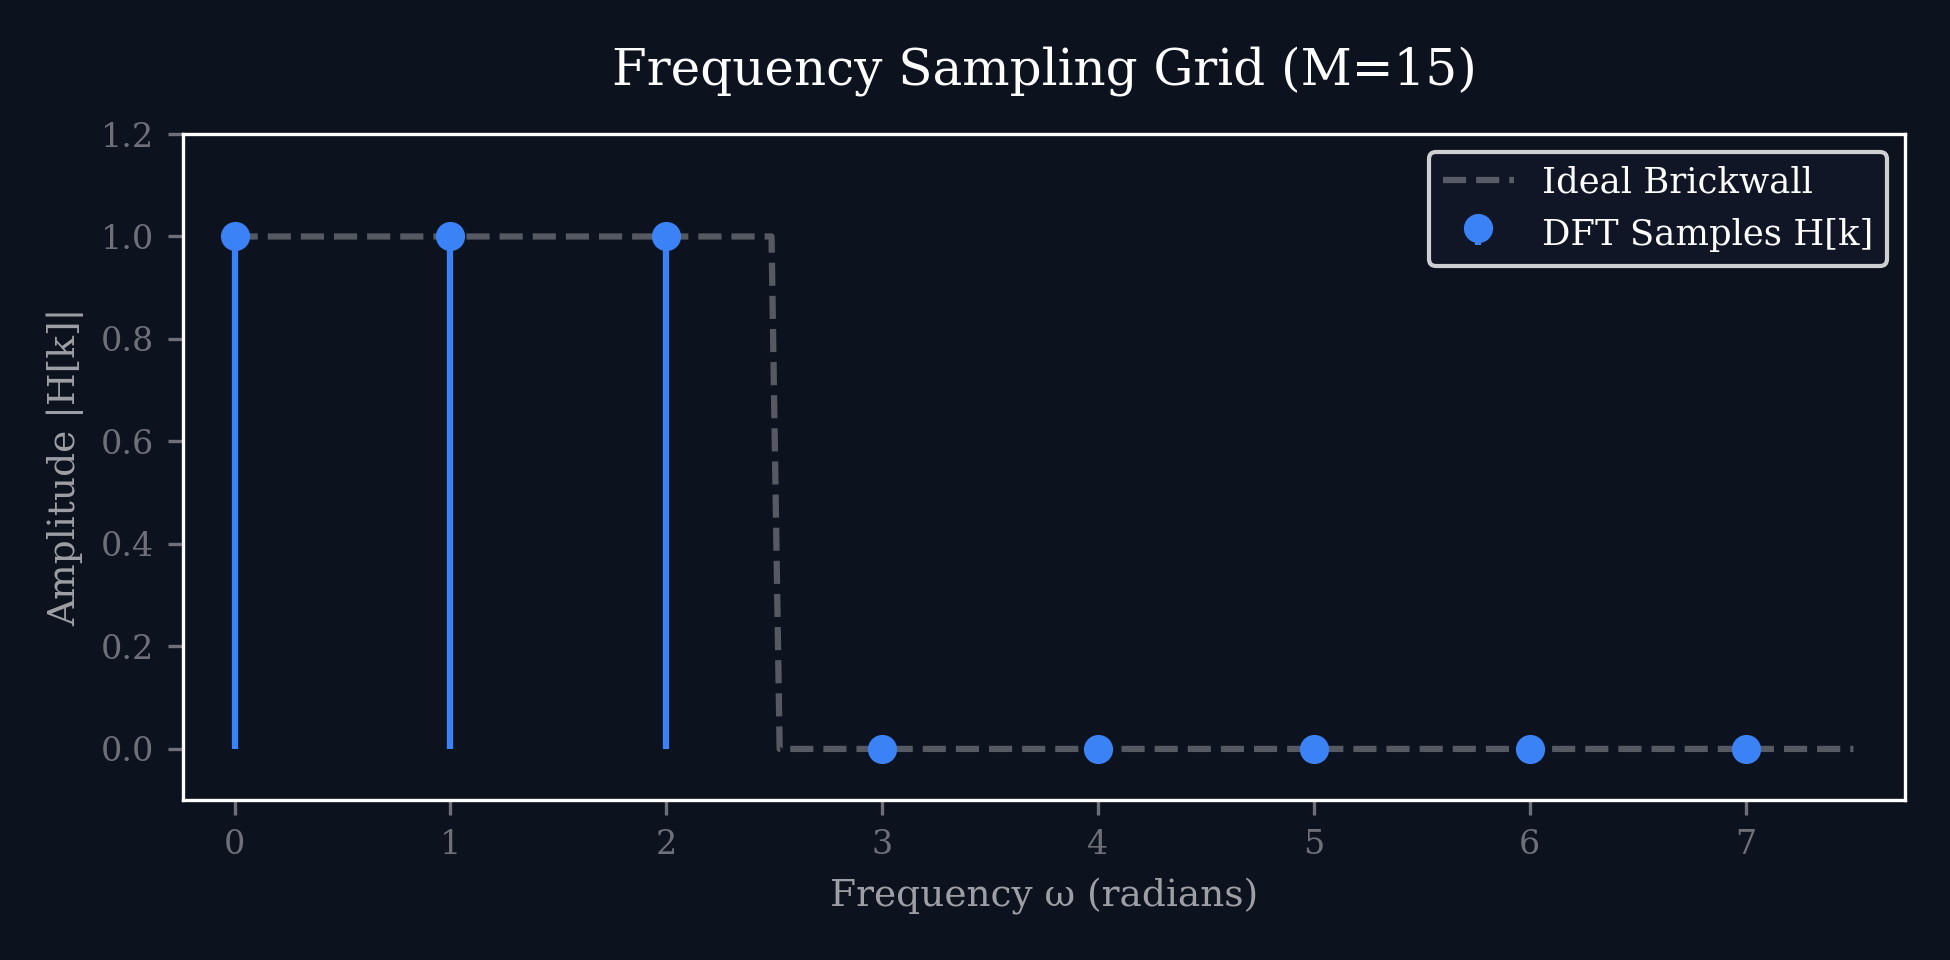
\includegraphics[width=0.6\textwidth]{images/freq_sampling_discrete.png}
\caption{Visualizing spectral envelope modeling discrete resonances.}
\label{fig:freq_sampling_discrete}
\end{figure}

\section{Cepstrum \& Homomorphic Analysis}
Speech $x[n] = e[n] * h[n]$.
Fourier transform and log magnitude:
\begin{equation}
\log |X(e^{j\omega})| = \log |E(e^{j\omega})| + \log |H(e^{j\omega})|
\end{equation}
Real cepstrum:
\begin{equation}
c[n] = \mathcal{F}^{-1}\{ \log |X(e^{j\omega})| \} = c_e[n] + c_h[n]
\end{equation}
$c_h[n]$ is at low quefrencies (vocal tract), $c_e[n]$ has a peak at $T_0$ (pitch).

\section{MFCC \& Pitch Detection}
\textbf{MFCC:} Window $\to$ FFT $\to$ Mel Filterbank $\to$ Log $\to$ DCT.

\textbf{Pitch Detection:}
\begin{itemize}
    \item \textbf{Autocorrelation:} $R_{xx}[k]$ peaks at $T_0$.
    \item \textbf{AMDF:} $D[k] = \sum |x[n] - x[n+k]|$ dips at $T_0$.
\end{itemize}

\begin{figure}[H]
\centering
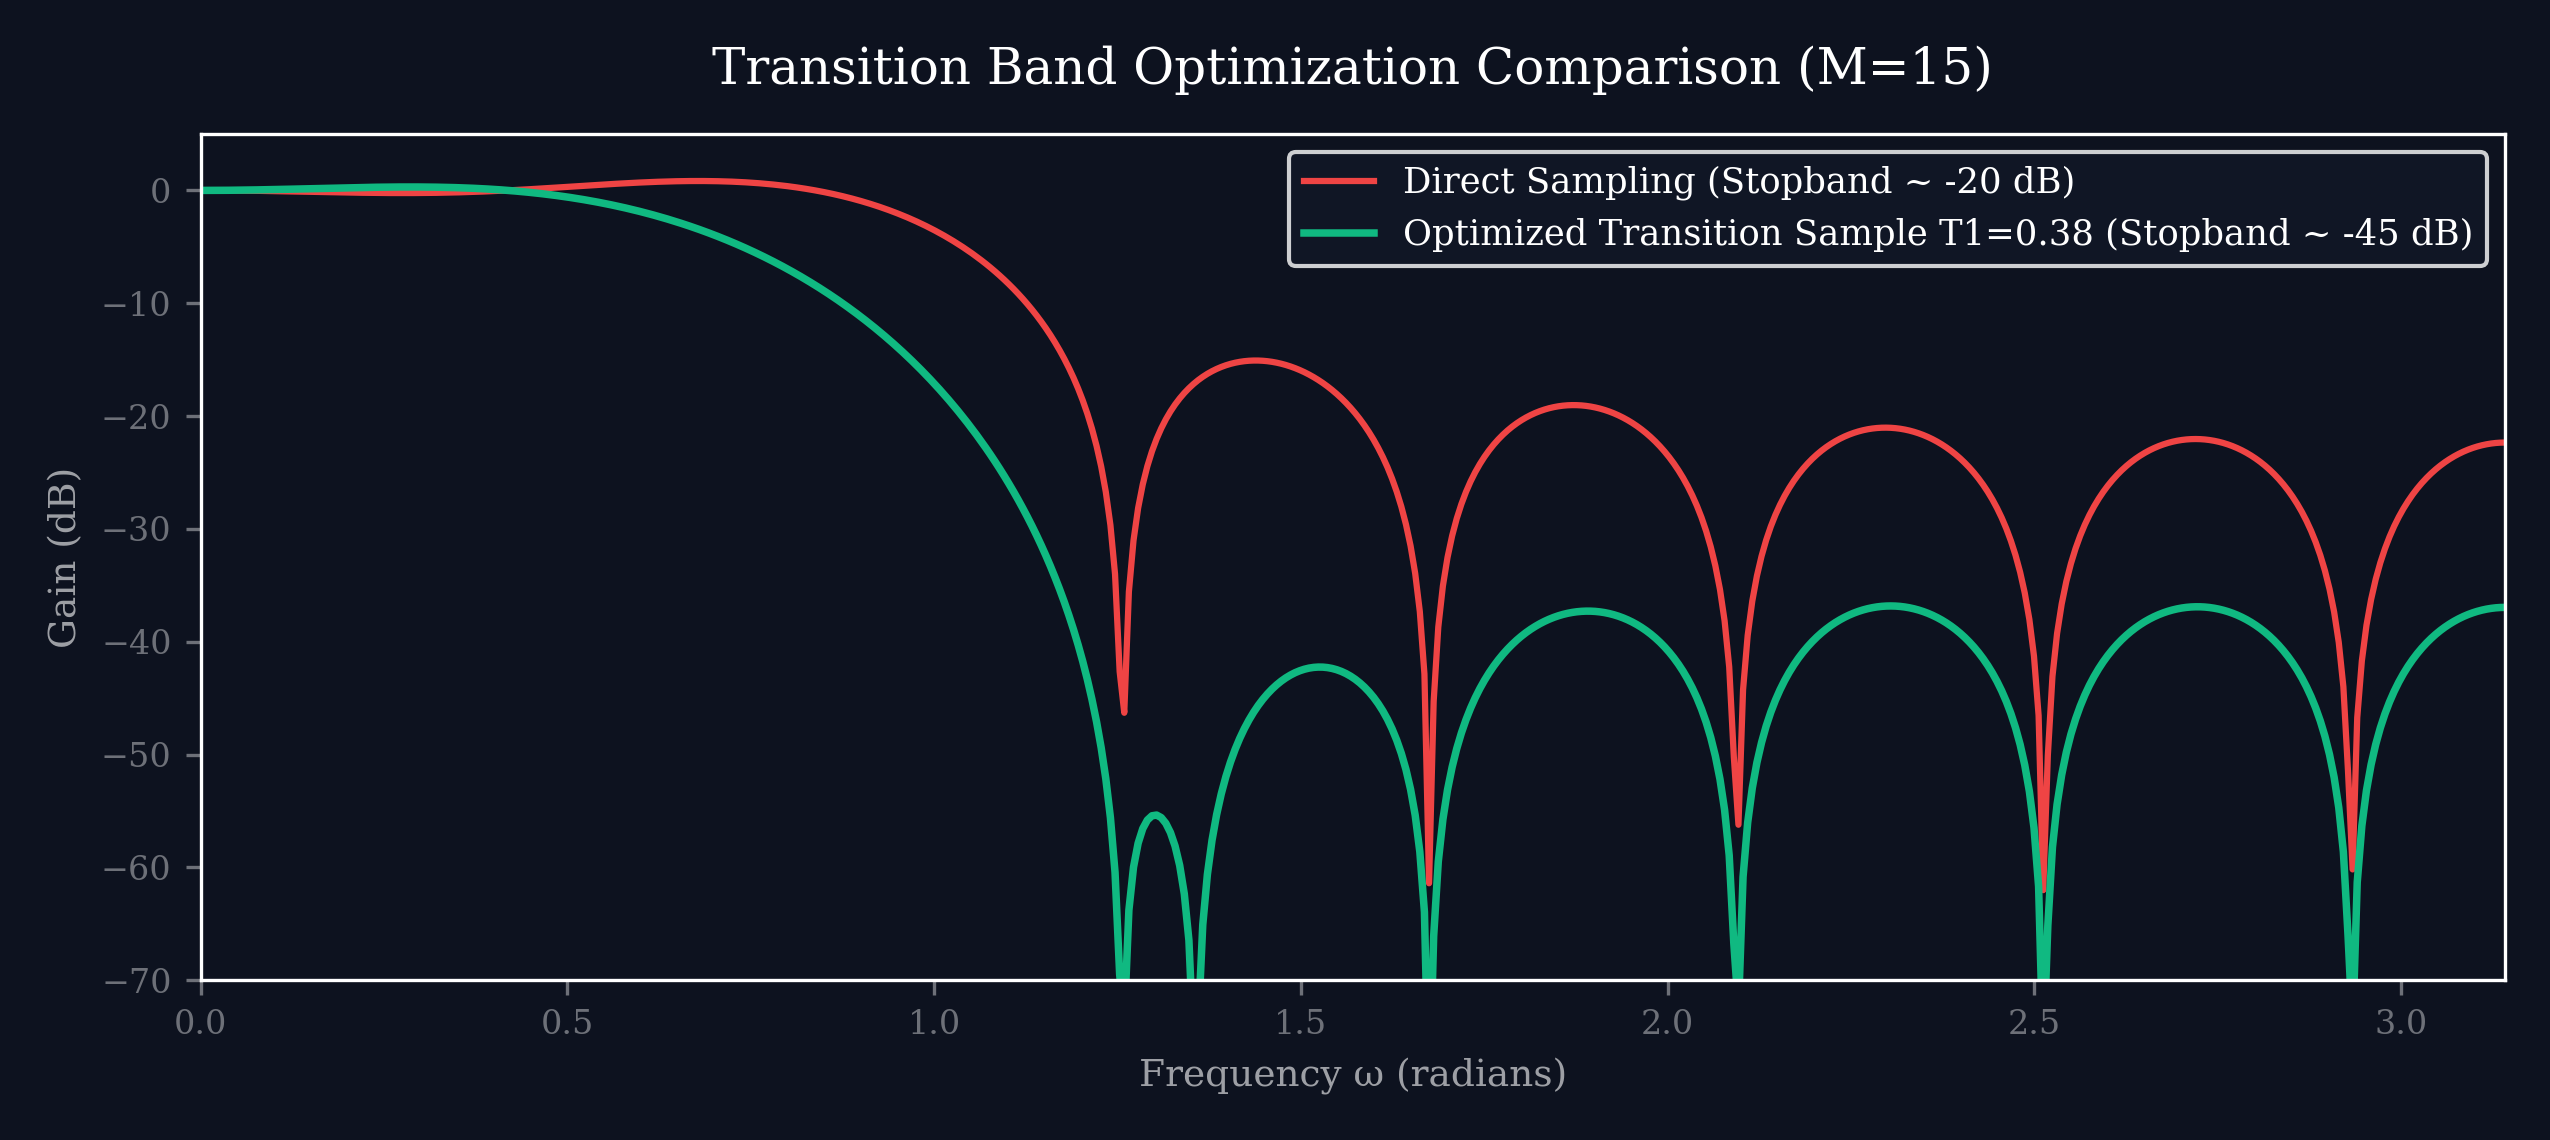
\includegraphics[width=0.75\textwidth]{images/transition_samples.png}
\caption{Analogous to transition bands, smooth pitch tracking avoids discontinuities.}
\label{fig:transition_samples}
\end{figure}

\section{Checkpoints}
\textbf{Q1: Derive $a_1$ and $E_1$ for $p=1$.} \\
\textit{Answer:} $a_1 R_{xx}[0] = -R_{xx}[1] \implies a_1 = -R_{xx}[1]/R_{xx}[0]$. \\
$E_1 = R_{xx}[0] + a_1 R_{xx}[1] = R_{xx}[0](1 - k_1^2)$.

\textbf{Q2: Why does the Cepstrum separate vocal tract and excitation?} \\
\textit{Answer:} Logarithm turns convolution into addition. The slow varying vocal tract $H$ appears at low quefrency, while the fast periodic excitation $E$ appears as a high quefrency peak.

\textbf{Q3: What guarantees $H(z)$ stability?} \\
\textit{Answer:} The Levinson-Durbin PARCOR coefficients $|k_m| < 1$ guarantee all poles of $1/A(z)$ are strictly inside the unit circle.

\end{document}
